In order to efficiently use the numerical scheme just described we will need to
implement the scheme using computational software.

\subsubsection{Discretized Solution}
We have implemented the numerical scheme described above in MATLAB which can be
used by calling the m-function \texttt{numerical\_scheme.m}. We will now
describe the parameters necessary to call the function, how the function
computes the solution, and the results outputted by the function. Please refer
to appendix \ref{append_analytical} for the function definition in MATLAB.

This m-function requires the following parameters to compute the numerical solution:
\begin{itemize}
  \item \texttt{f} - MATLAB function that represents the function $f$ in the differential equation $Lu = f$.
  \item \texttt{c} - A real number that represents the constant $c$ in the differential equation $Lu = f$.
  \item \texttt{initials} - An array with two elements representing the initial conditions in the problem
    $Lu=f$. The first element of the array is $\epsilon$ and the second element of the array is $\delta$.
  \item \texttt{interval} - An array with two elements representing the endpoints of the interval of definition in
    the problem $Lu = f$.
  \item \texttt{subintervals} - An integer that represents the number of subintervals with which to construct
    the uniform nodes on the interval of definition. This corresponds to an
    $h$-value of $1/\texttt{subintervals}$ on the grid $D_h$.
\end{itemize}

Calling the function as follows
\[
  \texttt{numerical\_scheme(f, c, initials, interval, subintervals)}
\]
returns the array \texttt{[x, u]} where \texttt{x} is an array whose elements are
the nodes on the grid $D_h$ and \texttt{u} is an array whose elements are the
numerical solution obtained by the scheme $L_h u^{(h)} = f^{(h)}$ evaluated on the
nodes of the grid.

From these parameters, after verifying that $c$ is a positive real number,
the function creates and assigns to \texttt{x} the uniform
nodes equally spaced on the passed interval with width 1/\texttt{subintervals}. We then
construct the  coefficient matrix \texttt{A} and the right-hand side vector \texttt{b} of the equation
in \eqref{matrix_system}. Finally, we then assign to \texttt{u} the solution vector
which is given by \texttt{initials(1), A\textbackslash b, initials(2)}.

Using this function then allows us to compute the numerical solution to the problem
$Lu = f$.

\subsubsection{Plotting}
Now that we have an implementation to compute the numerical approximation to the
exact solution to the problem $Lu =f$, we would like to also have a way to plot
that solution.

In order to achieve that goal, we have implemented a function that performs
linear spline interpolation where the interpolants are the values of the computed
approximate solution using the numerical scheme $L_h u^{(h)} = f^{(h)}$.

The m-function \texttt{plot\_interpolation.m} takes as input the output from the
m-function \texttt{numerical\_scheme.m}, i.e.\ the nodes \texttt{x} and the
solution vector \texttt{u}. This produces a figure that plots the original
vector \texttt{u} and the linear splines that interpolate the elements of the
vector \texttt{u}.

As the number of nodes increases, the plot of the solution becomes smoother as
can be seen in Figure \ref{example_plot}.

\begin{figure}[h!]
  \begin{center}
    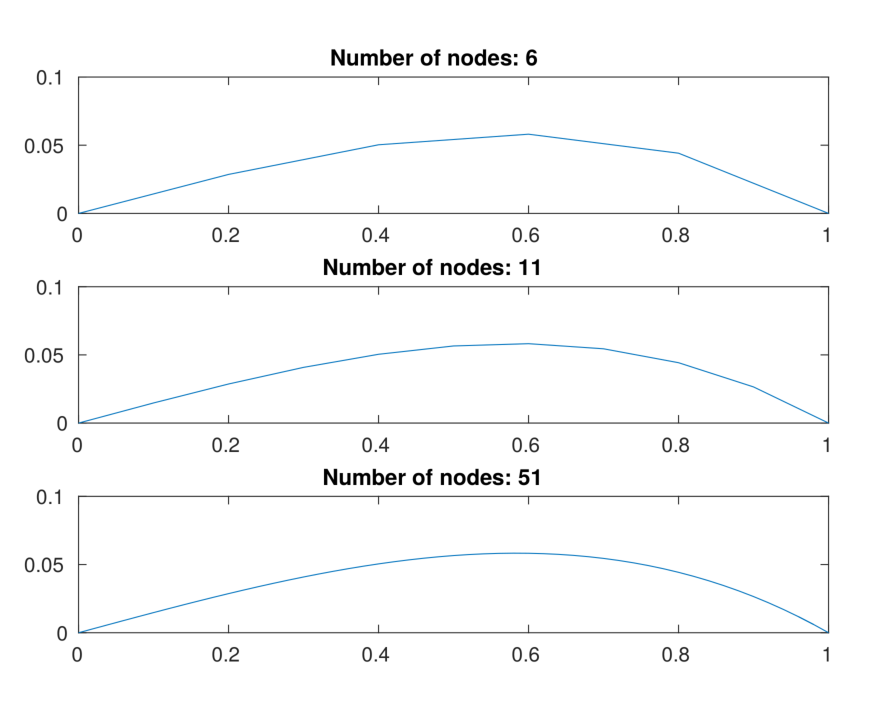
\includegraphics[scale=0.75]{example}
  \end{center}
  \caption{Plotted solution obtained from numerical scheme $L_h u^{(h)} = f^{(h)}$ for the problem $Lu = f$ with
    $f(x) = x$, $c =1$, and initial conditions $u(0) = 0$, $u(1) = 0$ for increasing number of nodes
    using the function \texttt{plot\_interpolation.m}.}\label{example_plot}
\end{figure}

We also have provided the m-function \texttt{linear\_interpolation.m} that evaluates
the solution obtained from the m-function \texttt{numerical\_scheme.m} for any $x$
on the interval of definition for the problem $Lu = f$. This is achieved
by evaluating the linear spline that interpolates the two nodes that contain
the point $x$ and returning that value.

The function definitions for \texttt{plot\_interpolation.m} and \texttt{linear\_interpolation.m}
can be found in Appendix \ref{append_plot}.